% FILE: figures/potential_landscape.tex
% Schematic potential landscape with thresholds

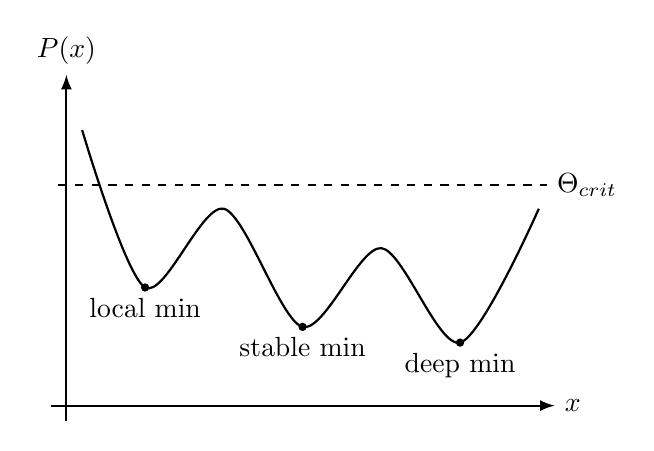
\begin{tikzpicture}[>=latex,thick,scale=1]
  % Axes
  \draw[->] (-0.2,0) -- (6.2,0) node[right] {$x$};
  \draw[->] (0,-0.2) -- (0,4.2) node[above] {$P(x)$};

  % Potential curve (hand-drawn with a few points)
  \draw[smooth,thick]
    plot coordinates {
      (0.2,3.5)
      (1.0,1.5)
      (2.0,2.5)
      (3.0,1.0)
      (4.0,2.0)
      (5.0,0.8)
      (6.0,2.5)
    };

  % Threshold line
  \draw[dashed] (-0.1,2.8) -- (6.1,2.8);
  \node[anchor=west] at (6.1,2.8) {$\Theta_{\text{crit}}$};

  % Local minima labels
  \fill (1.0,1.5) circle (1.5pt);
  \node[below] at (1.0,1.5) {local min};

  \fill (3.0,1.0) circle (1.5pt);
  \node[below] at (3.0,1.0) {stable min};

  \fill (5.0,0.8) circle (1.5pt);
  \node[below] at (5.0,0.8) {deep min};
\end{tikzpicture}

